\documentclass[aspectratio=169,10pt]{beamer}
\usetheme{Madrid}
\usecolortheme{whale}
\usepackage{pgfplots}
\pgfplotsset{compat=1.18}
\usepackage{booktabs}
\usepackage{amsmath}

\pgfplotsset{
  every axis/.style={
    width=6.5cm, height=5cm,
    grid=major, grid style={dashed,gray!40},
    mark size=1.5pt,
    xlabel={$p$},
    xmin=0, xmax=0.12,
    scaled ticks=false,
    yticklabel style={/pgf/number format/fixed},
    legend style={at={(0.5,1.03)}, anchor=south, font=\tiny},
  },
  black line/.style={
    smooth, thick, black,
  },
}

\title{Comparison of Shock Variances ($\omega$)}
\subtitle{$\omega=0.55$ vs.\ $\omega=0.15$ vs.\ $\omega=0.05$}
\author{}
\date{\today}

\begin{document}

\begin{frame}
  \titlepage
\end{frame}

% ============================================================
\section{Rationing}
% ============================================================

\begin{frame}{Rationing: $\omega$ comparison}
  \begin{columns}[T]
    \begin{column}{0.55\textwidth}
      \begin{figure}
        \centering
        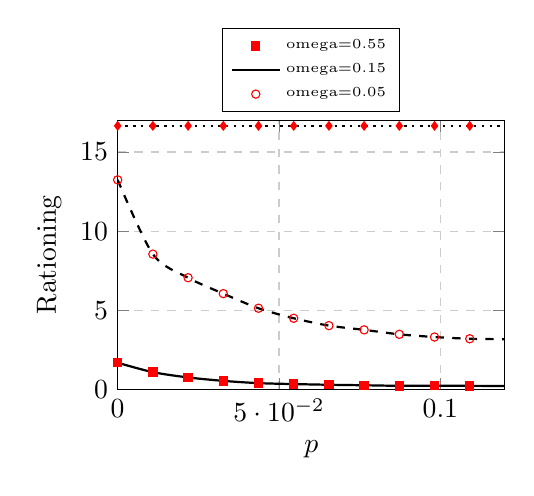
\begin{tikzpicture}
          \begin{axis}[
            ylabel={Rationing},
            ymin=0, ymax=17,
          ]
            \addplot[only marks, mark=square*, red] coordinates {
              (1e-05,1.6911) (0.01091909090909091,1.0958) (0.02182818181818182,0.7629) (0.03273727272727273,0.5452) (0.04364636363636364,0.4027) (0.05455545454545455,0.3433) (0.06546454545454546,0.2995) (0.07637363636363637,0.2684) (0.08728272727272728,0.2330) (0.09819181818181819,0.2379) (0.1091009090909091,0.2314) (0.12001,0.2219)
            };
            \addplot[black line] coordinates {
              (1e-05,1.6911) (0.01091909090909091,1.0958) (0.02182818181818182,0.7629) (0.03273727272727273,0.5452) (0.04364636363636364,0.4027) (0.05455545454545455,0.3433) (0.06546454545454546,0.2995) (0.07637363636363637,0.2684) (0.08728272727272728,0.2330) (0.09819181818181819,0.2379) (0.1091009090909091,0.2314) (0.12001,0.2219)
            };
            \addlegendentry{omega=0.55}
            \addplot[only marks, mark=o, red] coordinates {
              (1e-05,13.2403) (0.01091909090909091,8.5499) (0.02182818181818182,7.0592) (0.03273727272727273,6.0556) (0.04364636363636364,5.1320) (0.05455545454545455,4.5000) (0.06546454545454546,4.0350) (0.07637363636363637,3.7673) (0.08728272727272728,3.4860) (0.09819181818181819,3.3151) (0.1091009090909091,3.2052) (0.12001,3.1761)
            };
            \addplot[black line, dashed] coordinates {
              (1e-05,13.2403) (0.01091909090909091,8.5499) (0.02182818181818182,7.0592) (0.03273727272727273,6.0556) (0.04364636363636364,5.1320) (0.05455545454545455,4.5000) (0.06546454545454546,4.0350) (0.07637363636363637,3.7673) (0.08728272727272728,3.4860) (0.09819181818181819,3.3151) (0.1091009090909091,3.2052) (0.12001,3.1761)
            };
            \addlegendentry{omega=0.15}
            \addplot[only marks, mark=diamond*, red] coordinates {
              (1e-05,16.6500) (0.01091909090909091,16.6500) (0.02182818181818182,16.6500) (0.03273727272727273,16.6500) (0.04364636363636364,16.6500) (0.05455545454545455,16.6500) (0.06546454545454546,16.6500) (0.07637363636363637,16.6500) (0.08728272727272728,16.6500) (0.09819181818181819,16.6500) (0.1091009090909091,16.6500) (0.12001,16.6500)
            };
            \addplot[black line, dotted] coordinates {
              (1e-05,16.6500) (0.01091909090909091,16.6500) (0.02182818181818182,16.6500) (0.03273727272727273,16.6500) (0.04364636363636364,16.6500) (0.05455545454545455,16.6500) (0.06546454545454546,16.6500) (0.07637363636363637,16.6500) (0.08728272727272728,16.6500) (0.09819181818181819,16.6500) (0.1091009090909091,16.6500) (0.12001,16.6500)
            };
            \addlegendentry{omega=0.05}
          \end{axis}
        \end{tikzpicture}
      \end{figure}
    \end{column}
    \begin{column}{0.42\textwidth}
      \footnotesize\renewcommand{\arraystretch}{0.85}\setlength{\tabcolsep}{3pt}
      \begin{tabular}{lrrr}
        \toprule
        $p$ & $\omega=0.55$ & $\omega=0.15$ & $\omega=0.05$ \\
        \midrule
        0.00001 & 1.6911 & 13.2403 & 16.6500 \\
        0.011 & 1.0958 & 8.5499 & 16.6500 \\
        0.022 & 0.7629 & 7.0592 & 16.6500 \\
        0.033 & 0.5452 & 6.0556 & 16.6500 \\
        0.044 & 0.4027 & 5.1320 & 16.6500 \\
        0.055 & 0.3433 & 4.5000 & 16.6500 \\
        \textbf{0.065} & \textbf{0.2995} & \textbf{4.0350} & \textbf{16.6500} \\
        0.076 & 0.2684 & 3.7673 & 16.6500 \\
        0.087 & 0.2330 & 3.4860 & 16.6500 \\
        0.098 & 0.2379 & 3.3151 & 16.6500 \\
        0.109 & 0.2314 & 3.2052 & 16.6500 \\
        0.120 & 0.2219 & 3.1761 & 16.6500 \\
        \bottomrule
      \end{tabular}
    \end{column}
  \end{columns}
\end{frame}

% ============================================================
\section{Contagion}
% ============================================================

\begin{frame}{Contagion: $\omega$ comparison}
  \begin{columns}[T]
    \begin{column}{0.55\textwidth}
      \begin{figure}
        \centering
        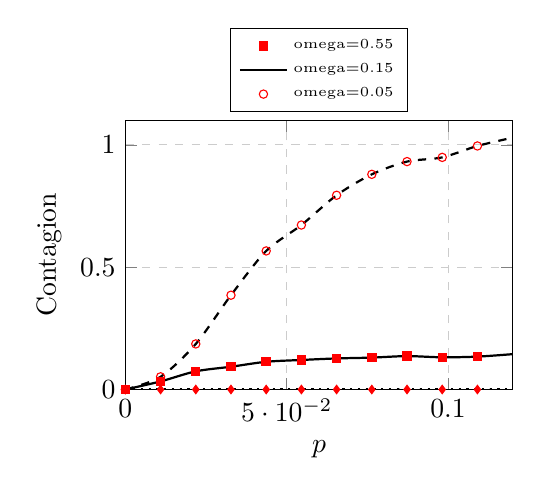
\begin{tikzpicture}
          \begin{axis}[
            ylabel={Contagion},
            ymin=0, ymax=1.1,
          ]
            \addplot[only marks, mark=square*, red] coordinates {
              (1e-05,0.0001) (0.01091909090909091,0.0331) (0.02182818181818182,0.0743) (0.03273727272727273,0.0931) (0.04364636363636364,0.1133) (0.05455545454545455,0.1207) (0.06546454545454546,0.1270) (0.07637363636363637,0.1304) (0.08728272727272728,0.1365) (0.09819181818181819,0.1316) (0.1091009090909091,0.1344) (0.12001,0.1445)
            };
            \addplot[black line] coordinates {
              (1e-05,0.0001) (0.01091909090909091,0.0331) (0.02182818181818182,0.0743) (0.03273727272727273,0.0931) (0.04364636363636364,0.1133) (0.05455545454545455,0.1207) (0.06546454545454546,0.1270) (0.07637363636363637,0.1304) (0.08728272727272728,0.1365) (0.09819181818181819,0.1316) (0.1091009090909091,0.1344) (0.12001,0.1445)
            };
            \addlegendentry{omega=0.55}
            \addplot[only marks, mark=o, red] coordinates {
              (1e-05,0.0000) (0.01091909090909091,0.0519) (0.02182818181818182,0.1862) (0.03273727272727273,0.3854) (0.04364636363636364,0.5663) (0.05455545454545455,0.6722) (0.06546454545454546,0.7938) (0.07637363636363637,0.8793) (0.08728272727272728,0.9314) (0.09819181818181819,0.9486) (0.1091009090909091,0.9953) (0.12001,1.0291)
            };
            \addplot[black line, dashed] coordinates {
              (1e-05,0.0000) (0.01091909090909091,0.0519) (0.02182818181818182,0.1862) (0.03273727272727273,0.3854) (0.04364636363636364,0.5663) (0.05455545454545455,0.6722) (0.06546454545454546,0.7938) (0.07637363636363637,0.8793) (0.08728272727272728,0.9314) (0.09819181818181819,0.9486) (0.1091009090909091,0.9953) (0.12001,1.0291)
            };
            \addlegendentry{omega=0.15}
            \addplot[only marks, mark=diamond*, red] coordinates {
              (1e-05,0.0000) (0.01091909090909091,0.0000) (0.02182818181818182,0.0000) (0.03273727272727273,0.0000) (0.04364636363636364,0.0000) (0.05455545454545455,0.0000) (0.06546454545454546,0.0000) (0.07637363636363637,0.0000) (0.08728272727272728,0.0000) (0.09819181818181819,0.0000) (0.1091009090909091,0.0000) (0.12001,0.0000)
            };
            \addplot[black line, dotted] coordinates {
              (1e-05,0.0000) (0.01091909090909091,0.0000) (0.02182818181818182,0.0000) (0.03273727272727273,0.0000) (0.04364636363636364,0.0000) (0.05455545454545455,0.0000) (0.06546454545454546,0.0000) (0.07637363636363637,0.0000) (0.08728272727272728,0.0000) (0.09819181818181819,0.0000) (0.1091009090909091,0.0000) (0.12001,0.0000)
            };
            \addlegendentry{omega=0.05}
          \end{axis}
        \end{tikzpicture}
      \end{figure}
    \end{column}
    \begin{column}{0.42\textwidth}
      \footnotesize\renewcommand{\arraystretch}{0.85}\setlength{\tabcolsep}{3pt}
      \begin{tabular}{lrrr}
        \toprule
        $p$ & $\omega=0.55$ & $\omega=0.15$ & $\omega=0.05$ \\
        \midrule
        0.00001 & 0.0001 & 0.0000 & 0.0000 \\
        0.011 & 0.0331 & 0.0519 & 0.0000 \\
        0.022 & 0.0743 & 0.1862 & 0.0000 \\
        0.033 & 0.0931 & 0.3854 & 0.0000 \\
        0.044 & 0.1133 & 0.5663 & 0.0000 \\
        0.055 & 0.1207 & 0.6722 & 0.0000 \\
        \textbf{0.065} & \textbf{0.1270} & \textbf{0.7938} & \textbf{0.0000} \\
        0.076 & 0.1304 & 0.8793 & 0.0000 \\
        0.087 & 0.1365 & 0.9314 & 0.0000 \\
        0.098 & 0.1316 & 0.9486 & 0.0000 \\
        0.109 & 0.1344 & 0.9953 & 0.0000 \\
        0.120 & 0.1445 & 1.0291 & 0.0000 \\
        \bottomrule
      \end{tabular}
    \end{column}
  \end{columns}
\end{frame}

% ============================================================
\section{Bad Debt}
% ============================================================

\begin{frame}{Bad Debt: $\omega$ comparison}
  \begin{columns}[T]
    \begin{column}{0.55\textwidth}
      \begin{figure}
        \centering
        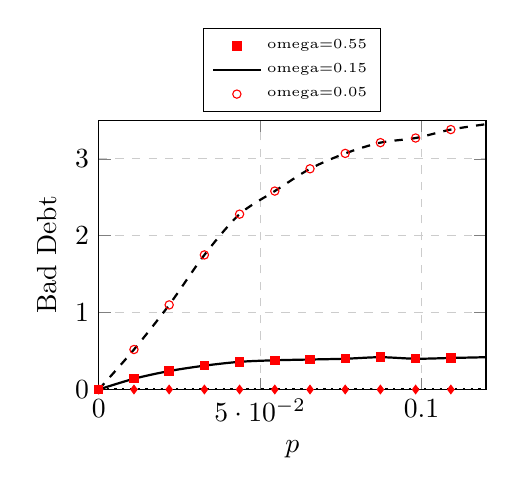
\begin{tikzpicture}
          \begin{axis}[
            ylabel={Bad Debt},
            ymin=0, ymax=3.5,
          ]
            \addplot[only marks, mark=square*, red] coordinates {
              (1e-05,0.00) (0.01091909090909091,0.14) (0.02182818181818182,0.24) (0.03273727272727273,0.31) (0.04364636363636364,0.36) (0.05455545454545455,0.38) (0.06546454545454546,0.39) (0.07637363636363637,0.40) (0.08728272727272728,0.42) (0.09819181818181819,0.40) (0.1091009090909091,0.41) (0.12001,0.42)
            };
            \addplot[black line] coordinates {
              (1e-05,0.00) (0.01091909090909091,0.14) (0.02182818181818182,0.24) (0.03273727272727273,0.31) (0.04364636363636364,0.36) (0.05455545454545455,0.38) (0.06546454545454546,0.39) (0.07637363636363637,0.40) (0.08728272727272728,0.42) (0.09819181818181819,0.40) (0.1091009090909091,0.41) (0.12001,0.42)
            };
            \addlegendentry{omega=0.55}
            \addplot[only marks, mark=o, red] coordinates {
              (1e-05,0.00) (0.01091909090909091,0.52) (0.02182818181818182,1.10) (0.03273727272727273,1.75) (0.04364636363636364,2.28) (0.05455545454545455,2.58) (0.06546454545454546,2.87) (0.07637363636363637,3.07) (0.08728272727272728,3.21) (0.09819181818181819,3.27) (0.1091009090909091,3.38) (0.12001,3.45)
            };
            \addplot[black line, dashed] coordinates {
              (1e-05,0.00) (0.01091909090909091,0.52) (0.02182818181818182,1.10) (0.03273727272727273,1.75) (0.04364636363636364,2.28) (0.05455545454545455,2.58) (0.06546454545454546,2.87) (0.07637363636363637,3.07) (0.08728272727272728,3.21) (0.09819181818181819,3.27) (0.1091009090909091,3.38) (0.12001,3.45)
            };
            \addlegendentry{omega=0.15}
            \addplot[only marks, mark=diamond*, red] coordinates {
              (1e-05,0.00) (0.01091909090909091,0.00) (0.02182818181818182,0.00) (0.03273727272727273,0.00) (0.04364636363636364,0.00) (0.05455545454545455,0.00) (0.06546454545454546,0.00) (0.07637363636363637,0.00) (0.08728272727272728,0.00) (0.09819181818181819,0.00) (0.1091009090909091,0.00) (0.12001,0.00)
            };
            \addplot[black line, dotted] coordinates {
              (1e-05,0.00) (0.01091909090909091,0.00) (0.02182818181818182,0.00) (0.03273727272727273,0.00) (0.04364636363636364,0.00) (0.05455545454545455,0.00) (0.06546454545454546,0.00) (0.07637363636363637,0.00) (0.08728272727272728,0.00) (0.09819181818181819,0.00) (0.1091009090909091,0.00) (0.12001,0.00)
            };
            \addlegendentry{omega=0.05}
          \end{axis}
        \end{tikzpicture}
      \end{figure}
    \end{column}
    \begin{column}{0.42\textwidth}
      \footnotesize\renewcommand{\arraystretch}{0.85}\setlength{\tabcolsep}{3pt}
      \begin{tabular}{lrrr}
        \toprule
        $p$ & $\omega=0.55$ & $\omega=0.15$ & $\omega=0.05$ \\
        \midrule
        0.00001 & 0.00 & 0.00 & 0.00 \\
        0.011 & 0.14 & 0.52 & 0.00 \\
        0.022 & 0.24 & 1.10 & 0.00 \\
        0.033 & 0.31 & 1.75 & 0.00 \\
        0.044 & 0.36 & 2.28 & 0.00 \\
        0.055 & 0.38 & 2.58 & 0.00 \\
        \textbf{0.065} & \textbf{0.39} & \textbf{2.87} & \textbf{0.00} \\
        0.076 & 0.40 & 3.07 & 0.00 \\
        0.087 & 0.42 & 3.21 & 0.00 \\
        0.098 & 0.40 & 3.27 & 0.00 \\
        0.109 & 0.41 & 3.38 & 0.00 \\
        0.120 & 0.42 & 3.45 & 0.00 \\
        \bottomrule
      \end{tabular}
    \end{column}
  \end{columns}
\end{frame}

% ============================================================
\section{Number of Loans}
% ============================================================

\begin{frame}{Num. Loans: $\omega$ comparison}
  \begin{columns}[T]
    \begin{column}{0.55\textwidth}
      \begin{figure}
        \centering
        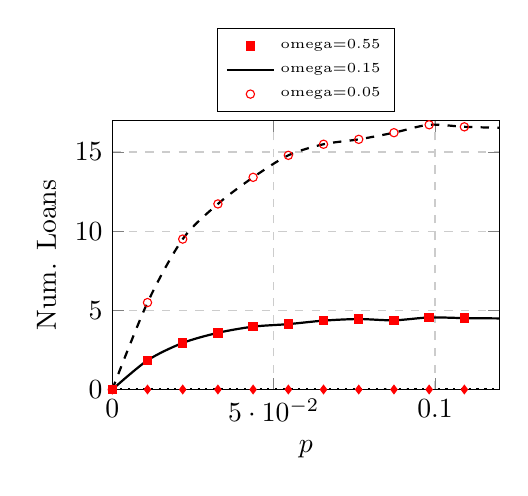
\begin{tikzpicture}
          \begin{axis}[
            ylabel={Num. Loans},
            ymin=0, ymax=17,
          ]
            \addplot[only marks, mark=square*, red] coordinates {
              (1e-05,0.00) (0.01091909090909091,1.84) (0.02182818181818182,2.94) (0.03273727272727273,3.58) (0.04364636363636364,3.97) (0.05455545454545455,4.13) (0.06546454545454546,4.35) (0.07637363636363637,4.45) (0.08728272727272728,4.37) (0.09819181818181819,4.55) (0.1091009090909091,4.51) (0.12001,4.49)
            };
            \addplot[black line] coordinates {
              (1e-05,0.00) (0.01091909090909091,1.84) (0.02182818181818182,2.94) (0.03273727272727273,3.58) (0.04364636363636364,3.97) (0.05455545454545455,4.13) (0.06546454545454546,4.35) (0.07637363636363637,4.45) (0.08728272727272728,4.37) (0.09819181818181819,4.55) (0.1091009090909091,4.51) (0.12001,4.49)
            };
            \addlegendentry{omega=0.55}
            \addplot[only marks, mark=o, red] coordinates {
              (1e-05,0.00) (0.01091909090909091,5.49) (0.02182818181818182,9.50) (0.03273727272727273,11.72) (0.04364636363636364,13.40) (0.05455545454545455,14.79) (0.06546454545454546,15.49) (0.07637363636363637,15.80) (0.08728272727272728,16.22) (0.09819181818181819,16.72) (0.1091009090909091,16.59) (0.12001,16.53)
            };
            \addplot[black line, dashed] coordinates {
              (1e-05,0.00) (0.01091909090909091,5.49) (0.02182818181818182,9.50) (0.03273727272727273,11.72) (0.04364636363636364,13.40) (0.05455545454545455,14.79) (0.06546454545454546,15.49) (0.07637363636363637,15.80) (0.08728272727272728,16.22) (0.09819181818181819,16.72) (0.1091009090909091,16.59) (0.12001,16.53)
            };
            \addlegendentry{omega=0.15}
            \addplot[only marks, mark=diamond*, red] coordinates {
              (1e-05,0.00) (0.01091909090909091,0.00) (0.02182818181818182,0.00) (0.03273727272727273,0.00) (0.04364636363636364,0.00) (0.05455545454545455,0.00) (0.06546454545454546,0.00) (0.07637363636363637,0.00) (0.08728272727272728,0.00) (0.09819181818181819,0.00) (0.1091009090909091,0.00) (0.12001,0.00)
            };
            \addplot[black line, dotted] coordinates {
              (1e-05,0.00) (0.01091909090909091,0.00) (0.02182818181818182,0.00) (0.03273727272727273,0.00) (0.04364636363636364,0.00) (0.05455545454545455,0.00) (0.06546454545454546,0.00) (0.07637363636363637,0.00) (0.08728272727272728,0.00) (0.09819181818181819,0.00) (0.1091009090909091,0.00) (0.12001,0.00)
            };
            \addlegendentry{omega=0.05}
          \end{axis}
        \end{tikzpicture}
      \end{figure}
    \end{column}
    \begin{column}{0.42\textwidth}
      \footnotesize\renewcommand{\arraystretch}{0.85}\setlength{\tabcolsep}{3pt}
      \begin{tabular}{lrrr}
        \toprule
        $p$ & $\omega=0.55$ & $\omega=0.15$ & $\omega=0.05$ \\
        \midrule
        0.00001 & 0.00 & 0.00 & 0.00 \\
        0.011 & 1.84 & 5.49 & 0.00 \\
        0.022 & 2.94 & 9.50 & 0.00 \\
        0.033 & 3.58 & 11.72 & 0.00 \\
        0.044 & 3.97 & 13.40 & 0.00 \\
        0.055 & 4.13 & 14.79 & 0.00 \\
        \textbf{0.065} & \textbf{4.35} & \textbf{15.49} & \textbf{0.00} \\
        0.076 & 4.45 & 15.80 & 0.00 \\
        0.087 & 4.37 & 16.22 & 0.00 \\
        0.098 & 4.55 & 16.72 & 0.00 \\
        0.109 & 4.51 & 16.59 & 0.00 \\
        0.120 & 4.49 & 16.53 & 0.00 \\
        \bottomrule
      \end{tabular}
    \end{column}
  \end{columns}
\end{frame}

% ============================================================
\section{Leverage}
% ============================================================

\begin{frame}{Leverage: $\omega$ comparison}
  \begin{columns}[T]
    \begin{column}{0.55\textwidth}
      \begin{figure}
        \centering
        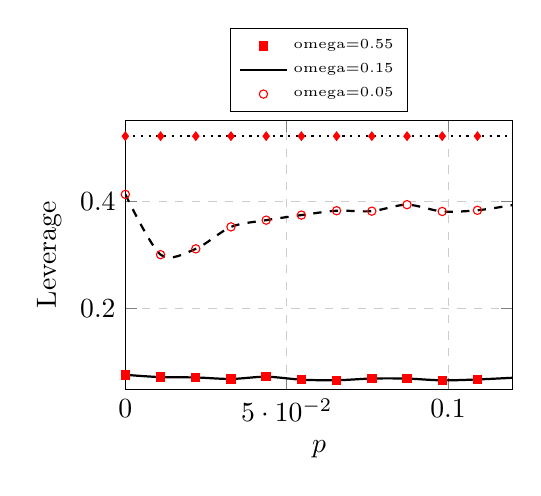
\begin{tikzpicture}
          \begin{axis}[
            ylabel={Leverage},
            ymin=0.05, ymax=0.55,
          ]
            \addplot[only marks, mark=square*, red] coordinates {
              (1e-05,0.0773) (0.01091909090909091,0.0730) (0.02182818181818182,0.0724) (0.03273727272727273,0.0696) (0.04364636363636364,0.0738) (0.05455545454545455,0.0683) (0.06546454545454546,0.0672) (0.07637363636363637,0.0704) (0.08728272727272728,0.0703) (0.09819181818181819,0.0670) (0.1091009090909091,0.0687) (0.12001,0.0718)
            };
            \addplot[black line] coordinates {
              (1e-05,0.0773) (0.01091909090909091,0.0730) (0.02182818181818182,0.0724) (0.03273727272727273,0.0696) (0.04364636363636364,0.0738) (0.05455545454545455,0.0683) (0.06546454545454546,0.0672) (0.07637363636363637,0.0704) (0.08728272727272728,0.0703) (0.09819181818181819,0.0670) (0.1091009090909091,0.0687) (0.12001,0.0718)
            };
            \addlegendentry{omega=0.55}
            \addplot[only marks, mark=o, red] coordinates {
              (1e-05,0.4125) (0.01091909090909091,0.3005) (0.02182818181818182,0.3113) (0.03273727272727273,0.3521) (0.04364636363636364,0.3646) (0.05455545454545455,0.3740) (0.06546454545454546,0.3821) (0.07637363636363637,0.3813) (0.08728272727272728,0.3934) (0.09819181818181819,0.3807) (0.1091009090909091,0.3829) (0.12001,0.3926)
            };
            \addplot[black line, dashed] coordinates {
              (1e-05,0.4125) (0.01091909090909091,0.3005) (0.02182818181818182,0.3113) (0.03273727272727273,0.3521) (0.04364636363636364,0.3646) (0.05455545454545455,0.3740) (0.06546454545454546,0.3821) (0.07637363636363637,0.3813) (0.08728272727272728,0.3934) (0.09819181818181819,0.3807) (0.1091009090909091,0.3829) (0.12001,0.3926)
            };
            \addlegendentry{omega=0.15}
            \addplot[only marks, mark=diamond*, red] coordinates {
              (1e-05,0.5206) (0.01091909090909091,0.5206) (0.02182818181818182,0.5206) (0.03273727272727273,0.5206) (0.04364636363636364,0.5206) (0.05455545454545455,0.5206) (0.06546454545454546,0.5206) (0.07637363636363637,0.5206) (0.08728272727272728,0.5206) (0.09819181818181819,0.5206) (0.1091009090909091,0.5206) (0.12001,0.5206)
            };
            \addplot[black line, dotted] coordinates {
              (1e-05,0.5206) (0.01091909090909091,0.5206) (0.02182818181818182,0.5206) (0.03273727272727273,0.5206) (0.04364636363636364,0.5206) (0.05455545454545455,0.5206) (0.06546454545454546,0.5206) (0.07637363636363637,0.5206) (0.08728272727272728,0.5206) (0.09819181818181819,0.5206) (0.1091009090909091,0.5206) (0.12001,0.5206)
            };
            \addlegendentry{omega=0.05}
          \end{axis}
        \end{tikzpicture}
      \end{figure}
    \end{column}
    \begin{column}{0.42\textwidth}
      \footnotesize\renewcommand{\arraystretch}{0.85}\setlength{\tabcolsep}{3pt}
      \begin{tabular}{lrrr}
        \toprule
        $p$ & $\omega=0.55$ & $\omega=0.15$ & $\omega=0.05$ \\
        \midrule
        0.00001 & 0.0773 & 0.4125 & 0.5206 \\
        0.011 & 0.0730 & 0.3005 & 0.5206 \\
        0.022 & 0.0724 & 0.3113 & 0.5206 \\
        0.033 & 0.0696 & 0.3521 & 0.5206 \\
        0.044 & 0.0738 & 0.3646 & 0.5206 \\
        0.055 & 0.0683 & 0.3740 & 0.5206 \\
        \textbf{0.065} & \textbf{0.0672} & \textbf{0.3821} & \textbf{0.5206} \\
        0.076 & 0.0704 & 0.3813 & 0.5206 \\
        0.087 & 0.0703 & 0.3934 & 0.5206 \\
        0.098 & 0.0670 & 0.3807 & 0.5206 \\
        0.109 & 0.0687 & 0.3829 & 0.5206 \\
        0.120 & 0.0718 & 0.3926 & 0.5206 \\
        \bottomrule
      \end{tabular}
    \end{column}
  \end{columns}
\end{frame}

% ============================================================
\section{Liquidity}
% ============================================================

\begin{frame}{Liquidity: $\omega$ comparison}
  \begin{columns}[T]
    \begin{column}{0.55\textwidth}
      \begin{figure}
        \centering
        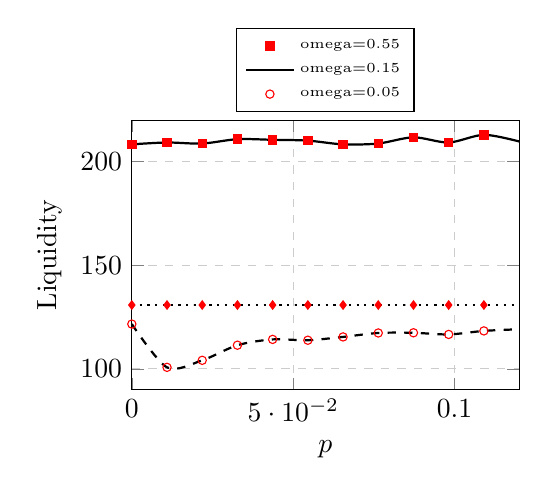
\begin{tikzpicture}
          \begin{axis}[
            ylabel={Liquidity},
            ymin=90, ymax=220,
          ]
            \addplot[only marks, mark=square*, red] coordinates {
              (1e-05,208.4) (0.01091909090909091,209.3) (0.02182818181818182,208.8) (0.03273727272727273,210.9) (0.04364636363636364,210.6) (0.05455545454545455,210.2) (0.06546454545454546,208.4) (0.07637363636363637,208.8) (0.08728272727272728,211.8) (0.09819181818181819,209.3) (0.1091009090909091,213.0) (0.12001,209.8)
            };
            \addplot[black line] coordinates {
              (1e-05,208.4) (0.01091909090909091,209.3) (0.02182818181818182,208.8) (0.03273727272727273,210.9) (0.04364636363636364,210.6) (0.05455545454545455,210.2) (0.06546454545454546,208.4) (0.07637363636363637,208.8) (0.08728272727272728,211.8) (0.09819181818181819,209.3) (0.1091009090909091,213.0) (0.12001,209.8)
            };
            \addlegendentry{omega=0.55}
            \addplot[only marks, mark=o, red] coordinates {
              (1e-05,121.6) (0.01091909090909091,100.7) (0.02182818181818182,104.1) (0.03273727272727273,111.4) (0.04364636363636364,114.2) (0.05455545454545455,113.8) (0.06546454545454546,115.4) (0.07637363636363637,117.3) (0.08728272727272728,117.4) (0.09819181818181819,116.6) (0.1091009090909091,118.3) (0.12001,119.1)
            };
            \addplot[black line, dashed] coordinates {
              (1e-05,121.6) (0.01091909090909091,100.7) (0.02182818181818182,104.1) (0.03273727272727273,111.4) (0.04364636363636364,114.2) (0.05455545454545455,113.8) (0.06546454545454546,115.4) (0.07637363636363637,117.3) (0.08728272727272728,117.4) (0.09819181818181819,116.6) (0.1091009090909091,118.3) (0.12001,119.1)
            };
            \addlegendentry{omega=0.15}
            \addplot[only marks, mark=diamond*, red] coordinates {
              (1e-05,130.8) (0.01091909090909091,130.8) (0.02182818181818182,130.8) (0.03273727272727273,130.8) (0.04364636363636364,130.8) (0.05455545454545455,130.8) (0.06546454545454546,130.8) (0.07637363636363637,130.8) (0.08728272727272728,130.8) (0.09819181818181819,130.8) (0.1091009090909091,130.8) (0.12001,130.8)
            };
            \addplot[black line, dotted] coordinates {
              (1e-05,130.8) (0.01091909090909091,130.8) (0.02182818181818182,130.8) (0.03273727272727273,130.8) (0.04364636363636364,130.8) (0.05455545454545455,130.8) (0.06546454545454546,130.8) (0.07637363636363637,130.8) (0.08728272727272728,130.8) (0.09819181818181819,130.8) (0.1091009090909091,130.8) (0.12001,130.8)
            };
            \addlegendentry{omega=0.05}
          \end{axis}
        \end{tikzpicture}
      \end{figure}
    \end{column}
    \begin{column}{0.42\textwidth}
      \footnotesize\renewcommand{\arraystretch}{0.85}\setlength{\tabcolsep}{3pt}
      \begin{tabular}{lrrr}
        \toprule
        $p$ & $\omega=0.55$ & $\omega=0.15$ & $\omega=0.05$ \\
        \midrule
        0.00001 & 208.4 & 121.6 & 130.8 \\
        0.011 & 209.3 & 100.7 & 130.8 \\
        0.022 & 208.8 & 104.1 & 130.8 \\
        0.033 & 210.9 & 111.4 & 130.8 \\
        0.044 & 210.6 & 114.2 & 130.8 \\
        0.055 & 210.2 & 113.8 & 130.8 \\
        \textbf{0.065} & \textbf{208.4} & \textbf{115.4} & \textbf{130.8} \\
        0.076 & 208.8 & 117.3 & 130.8 \\
        0.087 & 211.8 & 117.4 & 130.8 \\
        0.098 & 209.3 & 116.6 & 130.8 \\
        0.109 & 213.0 & 118.3 & 130.8 \\
        0.120 & 209.8 & 119.1 & 130.8 \\
        \bottomrule
      \end{tabular}
    \end{column}
  \end{columns}
\end{frame}

% ============================================================
\section{Deposits}
% ============================================================

\begin{frame}{Deposits: $\omega$ comparison}
  \begin{columns}[T]
    \begin{column}{0.55\textwidth}
      \begin{figure}
        \centering
        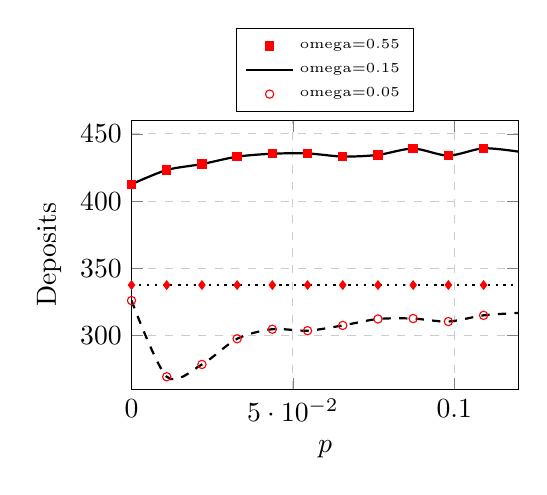
\begin{tikzpicture}
          \begin{axis}[
            ylabel={Deposits},
            ymin=260, ymax=460,
          ]
            \addplot[only marks, mark=square*, red] coordinates {
              (1e-05,412.5) (0.01091909090909091,423.1) (0.02182818181818182,427.5) (0.03273727272727273,433.0) (0.04364636363636364,435.2) (0.05455545454545455,435.4) (0.06546454545454546,433.1) (0.07637363636363637,434.3) (0.08728272727272728,439.0) (0.09819181818181819,433.8) (0.1091009090909091,439.2) (0.12001,436.7)
            };
            \addplot[black line] coordinates {
              (1e-05,412.5) (0.01091909090909091,423.1) (0.02182818181818182,427.5) (0.03273727272727273,433.0) (0.04364636363636364,435.2) (0.05455545454545455,435.4) (0.06546454545454546,433.1) (0.07637363636363637,434.3) (0.08728272727272728,439.0) (0.09819181818181819,433.8) (0.1091009090909091,439.2) (0.12001,436.7)
            };
            \addlegendentry{omega=0.55}
            \addplot[only marks, mark=o, red] coordinates {
              (1e-05,326.1) (0.01091909090909091,269.5) (0.02182818181818182,278.6) (0.03273727272727273,297.7) (0.04364636363636364,304.8) (0.05455545454545455,303.7) (0.06546454545454546,307.6) (0.07637363636363637,312.4) (0.08728272727272728,312.7) (0.09819181818181819,310.5) (0.1091009090909091,315.1) (0.12001,316.9)
            };
            \addplot[black line, dashed] coordinates {
              (1e-05,326.1) (0.01091909090909091,269.5) (0.02182818181818182,278.6) (0.03273727272727273,297.7) (0.04364636363636364,304.8) (0.05455545454545455,303.7) (0.06546454545454546,307.6) (0.07637363636363637,312.4) (0.08728272727272728,312.7) (0.09819181818181819,310.5) (0.1091009090909091,315.1) (0.12001,316.9)
            };
            \addlegendentry{omega=0.15}
            \addplot[only marks, mark=diamond*, red] coordinates {
              (1e-05,337.6) (0.01091909090909091,337.6) (0.02182818181818182,337.6) (0.03273727272727273,337.6) (0.04364636363636364,337.6) (0.05455545454545455,337.6) (0.06546454545454546,337.6) (0.07637363636363637,337.6) (0.08728272727272728,337.6) (0.09819181818181819,337.6) (0.1091009090909091,337.6) (0.12001,337.6)
            };
            \addplot[black line, dotted] coordinates {
              (1e-05,337.6) (0.01091909090909091,337.6) (0.02182818181818182,337.6) (0.03273727272727273,337.6) (0.04364636363636364,337.6) (0.05455545454545455,337.6) (0.06546454545454546,337.6) (0.07637363636363637,337.6) (0.08728272727272728,337.6) (0.09819181818181819,337.6) (0.1091009090909091,337.6) (0.12001,337.6)
            };
            \addlegendentry{omega=0.05}
          \end{axis}
        \end{tikzpicture}
      \end{figure}
    \end{column}
    \begin{column}{0.42\textwidth}
      \footnotesize\renewcommand{\arraystretch}{0.85}\setlength{\tabcolsep}{3pt}
      \begin{tabular}{lrrr}
        \toprule
        $p$ & $\omega=0.55$ & $\omega=0.15$ & $\omega=0.05$ \\
        \midrule
        0.00001 & 412.5 & 326.1 & 337.6 \\
        0.011 & 423.1 & 269.5 & 337.6 \\
        0.022 & 427.5 & 278.6 & 337.6 \\
        0.033 & 433.0 & 297.7 & 337.6 \\
        0.044 & 435.2 & 304.8 & 337.6 \\
        0.055 & 435.4 & 303.7 & 337.6 \\
        \textbf{0.065} & \textbf{433.1} & \textbf{307.6} & \textbf{337.6} \\
        0.076 & 434.3 & 312.4 & 337.6 \\
        0.087 & 439.0 & 312.7 & 337.6 \\
        0.098 & 433.8 & 310.5 & 337.6 \\
        0.109 & 439.2 & 315.1 & 337.6 \\
        0.120 & 436.7 & 316.9 & 337.6 \\
        \bottomrule
      \end{tabular}
    \end{column}
  \end{columns}
\end{frame}

% ============================================================
\section{Market Power}
% ============================================================

\begin{frame}{Market Power ($\psi$): $\omega$ comparison}
  \begin{columns}[T]
    \begin{column}{0.55\textwidth}
      \begin{figure}
        \centering
        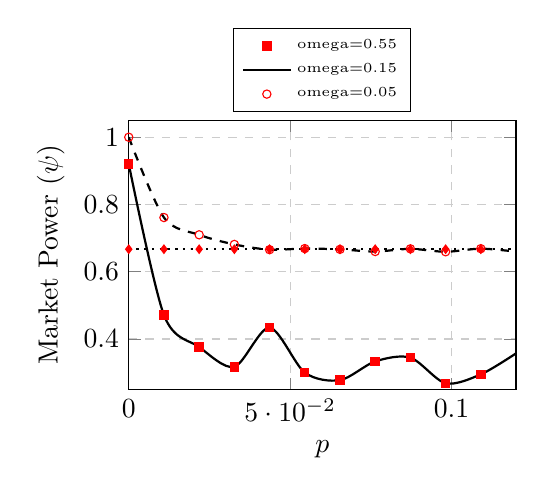
\begin{tikzpicture}
          \begin{axis}[
            ylabel={Market Power ($\psi$)},
            ymin=0.25, ymax=1.05,
          ]
            \addplot[only marks, mark=square*, red] coordinates {
              (1e-05,0.9204) (0.01091909090909091,0.4712) (0.02182818181818182,0.3765) (0.03273727272727273,0.3175) (0.04364636363636364,0.4340) (0.05455545454545455,0.3004) (0.06546454545454546,0.2778) (0.07637363636363637,0.3335) (0.08728272727272728,0.3448) (0.09819181818181819,0.2687) (0.1091009090909091,0.2950) (0.12001,0.3574)
            };
            \addplot[black line] coordinates {
              (1e-05,0.9204) (0.01091909090909091,0.4712) (0.02182818181818182,0.3765) (0.03273727272727273,0.3175) (0.04364636363636364,0.4340) (0.05455545454545455,0.3004) (0.06546454545454546,0.2778) (0.07637363636363637,0.3335) (0.08728272727272728,0.3448) (0.09819181818181819,0.2687) (0.1091009090909091,0.2950) (0.12001,0.3574)
            };
            \addlegendentry{omega=0.55}
            \addplot[only marks, mark=o, red] coordinates {
              (1e-05,0.9998) (0.01091909090909091,0.7611) (0.02182818181818182,0.7098) (0.03273727272727273,0.6812) (0.04364636363636364,0.6656) (0.05455545454545455,0.6689) (0.06546454545454546,0.6665) (0.07637363636363637,0.6601) (0.08728272727272728,0.6681) (0.09819181818181819,0.6594) (0.1091009090909091,0.6686) (0.12001,0.6597)
            };
            \addplot[black line, dashed] coordinates {
              (1e-05,0.9998) (0.01091909090909091,0.7611) (0.02182818181818182,0.7098) (0.03273727272727273,0.6812) (0.04364636363636364,0.6656) (0.05455545454545455,0.6689) (0.06546454545454546,0.6665) (0.07637363636363637,0.6601) (0.08728272727272728,0.6681) (0.09819181818181819,0.6594) (0.1091009090909091,0.6686) (0.12001,0.6597)
            };
            \addlegendentry{omega=0.15}
            \addplot[only marks, mark=diamond*, red] coordinates {
              (1e-05,0.6670) (0.01091909090909091,0.6670) (0.02182818181818182,0.6670) (0.03273727272727273,0.6670) (0.04364636363636364,0.6670) (0.05455545454545455,0.6670) (0.06546454545454546,0.6670) (0.07637363636363637,0.6670) (0.08728272727272728,0.6670) (0.09819181818181819,0.6670) (0.1091009090909091,0.6670) (0.12001,0.6670)
            };
            \addplot[black line, dotted] coordinates {
              (1e-05,0.6670) (0.01091909090909091,0.6670) (0.02182818181818182,0.6670) (0.03273727272727273,0.6670) (0.04364636363636364,0.6670) (0.05455545454545455,0.6670) (0.06546454545454546,0.6670) (0.07637363636363637,0.6670) (0.08728272727272728,0.6670) (0.09819181818181819,0.6670) (0.1091009090909091,0.6670) (0.12001,0.6670)
            };
            \addlegendentry{omega=0.05}
          \end{axis}
        \end{tikzpicture}
      \end{figure}
    \end{column}
    \begin{column}{0.42\textwidth}
      \footnotesize\renewcommand{\arraystretch}{0.85}\setlength{\tabcolsep}{3pt}
      \begin{tabular}{lrrr}
        \toprule
        $p$ & $\omega=0.55$ & $\omega=0.15$ & $\omega=0.05$ \\
        \midrule
        0.00001 & 0.9204 & 0.9998 & 0.6670 \\
        0.011 & 0.4712 & 0.7611 & 0.6670 \\
        0.022 & 0.3765 & 0.7098 & 0.6670 \\
        0.033 & 0.3175 & 0.6812 & 0.6670 \\
        0.044 & 0.4340 & 0.6656 & 0.6670 \\
        0.055 & 0.3004 & 0.6689 & 0.6670 \\
        \textbf{0.065} & \textbf{0.2778} & \textbf{0.6665} & \textbf{0.6670} \\
        0.076 & 0.3335 & 0.6601 & 0.6670 \\
        0.087 & 0.3448 & 0.6681 & 0.6670 \\
        0.098 & 0.2687 & 0.6594 & 0.6670 \\
        0.109 & 0.2950 & 0.6686 & 0.6670 \\
        0.120 & 0.3574 & 0.6597 & 0.6670 \\
        \bottomrule
      \end{tabular}
    \end{column}
  \end{columns}
\end{frame}

% ============================================================
\section{Interest Rate}
% ============================================================

\begin{frame}{Interest Rate ($ir$): $\omega$ comparison}
  \begin{columns}[T]
    \begin{column}{0.55\textwidth}
      \begin{figure}
        \centering
        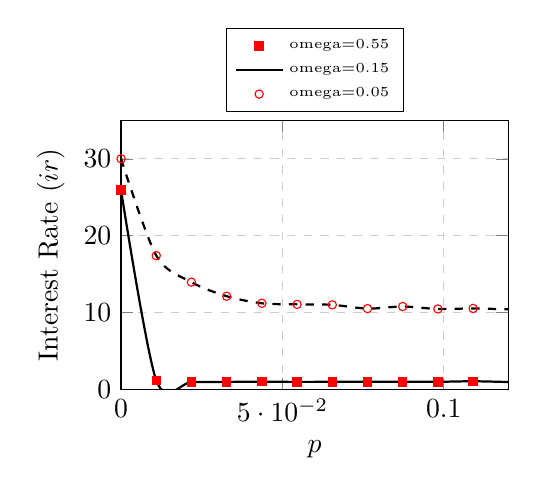
\begin{tikzpicture}
          \begin{axis}[
            ylabel={Interest Rate ($ir$)},
            ymin=0, ymax=35,
          ]
            \addplot[only marks, mark=square*, red] coordinates {
              (1e-05,25.92) (0.01091909090909091,1.19) (0.02182818181818182,0.98) (0.03273727272727273,0.99) (0.04364636363636364,1.01) (0.05455545454545455,0.99) (0.06546454545454546,1.00) (0.07637363636363637,1.00) (0.08728272727272728,1.00) (0.09819181818181819,1.00) (0.1091009090909091,1.07) (0.12001,0.97)
            };
            \addplot[black line] coordinates {
              (1e-05,25.92) (0.01091909090909091,1.19) (0.02182818181818182,0.98) (0.03273727272727273,0.99) (0.04364636363636364,1.01) (0.05455545454545455,0.99) (0.06546454545454546,1.00) (0.07637363636363637,1.00) (0.08728272727272728,1.00) (0.09819181818181819,1.00) (0.1091009090909091,1.07) (0.12001,0.97)
            };
            \addlegendentry{omega=0.55}
            \addplot[only marks, mark=o, red] coordinates {
              (1e-05,30.00) (0.01091909090909091,17.41) (0.02182818181818182,13.96) (0.03273727272727273,12.13) (0.04364636363636364,11.21) (0.05455545454545455,11.07) (0.06546454545454546,11.01) (0.07637363636363637,10.52) (0.08728272727272728,10.79) (0.09819181818181819,10.47) (0.1091009090909091,10.54) (0.12001,10.42)
            };
            \addplot[black line, dashed] coordinates {
              (1e-05,30.00) (0.01091909090909091,17.41) (0.02182818181818182,13.96) (0.03273727272727273,12.13) (0.04364636363636364,11.21) (0.05455545454545455,11.07) (0.06546454545454546,11.01) (0.07637363636363637,10.52) (0.08728272727272728,10.79) (0.09819181818181819,10.47) (0.1091009090909091,10.54) (0.12001,10.42)
            };
            \addlegendentry{omega=0.15}
            \addplot[only marks, mark=diamond*, red] coordinates {
              (1e-05,nan) (0.01091909090909091,nan) (0.02182818181818182,nan) (0.03273727272727273,nan) (0.04364636363636364,nan) (0.05455545454545455,nan) (0.06546454545454546,nan) (0.07637363636363637,nan) (0.08728272727272728,nan) (0.09819181818181819,nan) (0.1091009090909091,nan) (0.12001,nan)
            };
            \addplot[black line, dotted] coordinates {
              (1e-05,nan) (0.01091909090909091,nan) (0.02182818181818182,nan) (0.03273727272727273,nan) (0.04364636363636364,nan) (0.05455545454545455,nan) (0.06546454545454546,nan) (0.07637363636363637,nan) (0.08728272727272728,nan) (0.09819181818181819,nan) (0.1091009090909091,nan) (0.12001,nan)
            };
            \addlegendentry{omega=0.05}
          \end{axis}
        \end{tikzpicture}
      \end{figure}
    \end{column}
    \begin{column}{0.42\textwidth}
      \footnotesize\renewcommand{\arraystretch}{0.85}\setlength{\tabcolsep}{3pt}
      \begin{tabular}{lrrr}
        \toprule
        $p$ & $\omega=0.55$ & $\omega=0.15$ & $\omega=0.05$ \\
        \midrule
        0.00001 & 25.92 & 30.00 & nan \\
        0.011 & 1.19 & 17.41 & nan \\
        0.022 & 0.98 & 13.96 & nan \\
        0.033 & 0.99 & 12.13 & nan \\
        0.044 & 1.01 & 11.21 & nan \\
        0.055 & 0.99 & 11.07 & nan \\
        \textbf{0.065} & \textbf{1.00} & \textbf{11.01} & \textbf{nan} \\
        0.076 & 1.00 & 10.52 & nan \\
        0.087 & 1.00 & 10.79 & nan \\
        0.098 & 1.00 & 10.47 & nan \\
        0.109 & 1.07 & 10.54 & nan \\
        0.120 & 0.97 & 10.42 & nan \\
        \bottomrule
      \end{tabular}
    \end{column}
  \end{columns}
\end{frame}

% ============================================================
\section{Loans}
% ============================================================

\begin{frame}{Loans: $\omega$ comparison}
  \begin{columns}[T]
    \begin{column}{0.55\textwidth}
      \begin{figure}
        \centering
        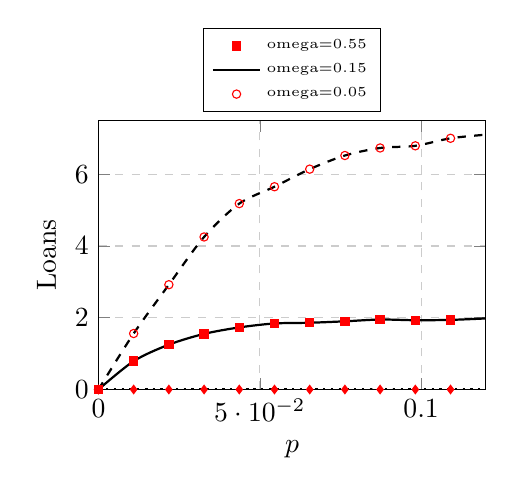
\begin{tikzpicture}
          \begin{axis}[
            ylabel={Loans},
            ymin=0, ymax=7.5,
          ]
            \addplot[only marks, mark=square*, red] coordinates {
              (1e-05,0.00) (0.01091909090909091,0.79) (0.02182818181818182,1.25) (0.03273727272727273,1.55) (0.04364636363636364,1.73) (0.05455545454545455,1.84) (0.06546454545454546,1.86) (0.07637363636363637,1.90) (0.08728272727272728,1.95) (0.09819181818181819,1.93) (0.1091009090909091,1.94) (0.12001,1.98)
            };
            \addplot[black line] coordinates {
              (1e-05,0.00) (0.01091909090909091,0.79) (0.02182818181818182,1.25) (0.03273727272727273,1.55) (0.04364636363636364,1.73) (0.05455545454545455,1.84) (0.06546454545454546,1.86) (0.07637363636363637,1.90) (0.08728272727272728,1.95) (0.09819181818181819,1.93) (0.1091009090909091,1.94) (0.12001,1.98)
            };
            \addlegendentry{omega=0.55}
            \addplot[only marks, mark=o, red] coordinates {
              (1e-05,0.00) (0.01091909090909091,1.56) (0.02182818181818182,2.92) (0.03273727272727273,4.25) (0.04364636363636364,5.18) (0.05455545454545455,5.65) (0.06546454545454546,6.14) (0.07637363636363637,6.52) (0.08728272727272728,6.73) (0.09819181818181819,6.79) (0.1091009090909091,7.00) (0.12001,7.10)
            };
            \addplot[black line, dashed] coordinates {
              (1e-05,0.00) (0.01091909090909091,1.56) (0.02182818181818182,2.92) (0.03273727272727273,4.25) (0.04364636363636364,5.18) (0.05455545454545455,5.65) (0.06546454545454546,6.14) (0.07637363636363637,6.52) (0.08728272727272728,6.73) (0.09819181818181819,6.79) (0.1091009090909091,7.00) (0.12001,7.10)
            };
            \addlegendentry{omega=0.15}
            \addplot[only marks, mark=diamond*, red] coordinates {
              (1e-05,0.00) (0.01091909090909091,0.00) (0.02182818181818182,0.00) (0.03273727272727273,0.00) (0.04364636363636364,0.00) (0.05455545454545455,0.00) (0.06546454545454546,0.00) (0.07637363636363637,0.00) (0.08728272727272728,0.00) (0.09819181818181819,0.00) (0.1091009090909091,0.00) (0.12001,0.00)
            };
            \addplot[black line, dotted] coordinates {
              (1e-05,0.00) (0.01091909090909091,0.00) (0.02182818181818182,0.00) (0.03273727272727273,0.00) (0.04364636363636364,0.00) (0.05455545454545455,0.00) (0.06546454545454546,0.00) (0.07637363636363637,0.00) (0.08728272727272728,0.00) (0.09819181818181819,0.00) (0.1091009090909091,0.00) (0.12001,0.00)
            };
            \addlegendentry{omega=0.05}
          \end{axis}
        \end{tikzpicture}
      \end{figure}
    \end{column}
    \begin{column}{0.42\textwidth}
      \footnotesize\renewcommand{\arraystretch}{0.85}\setlength{\tabcolsep}{3pt}
      \begin{tabular}{lrrr}
        \toprule
        $p$ & $\omega=0.55$ & $\omega=0.15$ & $\omega=0.05$ \\
        \midrule
        0.00001 & 0.00 & 0.00 & 0.00 \\
        0.011 & 0.79 & 1.56 & 0.00 \\
        0.022 & 1.25 & 2.92 & 0.00 \\
        0.033 & 1.55 & 4.25 & 0.00 \\
        0.044 & 1.73 & 5.18 & 0.00 \\
        0.055 & 1.84 & 5.65 & 0.00 \\
        \textbf{0.065} & \textbf{1.86} & \textbf{6.14} & \textbf{0.00} \\
        0.076 & 1.90 & 6.52 & 0.00 \\
        0.087 & 1.95 & 6.73 & 0.00 \\
        0.098 & 1.93 & 6.79 & 0.00 \\
        0.109 & 1.94 & 7.00 & 0.00 \\
        0.120 & 1.98 & 7.10 & 0.00 \\
        \bottomrule
      \end{tabular}
    \end{column}
  \end{columns}
\end{frame}

% ============================================================
\section{Probability of Bankruptcy}
% ============================================================

\begin{frame}{Probability of Bankruptcy ($p_b$): $\omega$ comparison}
  \begin{columns}[T]
    \begin{column}{0.55\textwidth}
      \begin{figure}
        \centering
        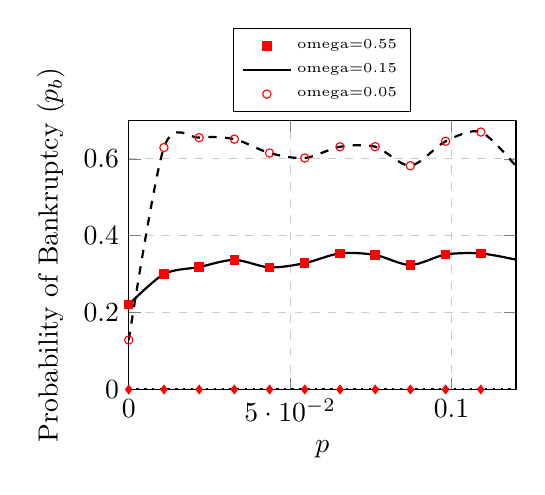
\begin{tikzpicture}
          \begin{axis}[
            ylabel={Probability of Bankruptcy ($p_b$)},
            ymin=0, ymax=0.7,
          ]
            \addplot[only marks, mark=square*, red] coordinates {
              (1e-05,0.2209) (0.01091909090909091,0.3002) (0.02182818181818182,0.3185) (0.03273727272727273,0.3371) (0.04364636363636364,0.3175) (0.05455545454545455,0.3286) (0.06546454545454546,0.3541) (0.07637363636363637,0.3499) (0.08728272727272728,0.3238) (0.09819181818181819,0.3510) (0.1091009090909091,0.3538) (0.12001,0.3377)
            };
            \addplot[black line] coordinates {
              (1e-05,0.2209) (0.01091909090909091,0.3002) (0.02182818181818182,0.3185) (0.03273727272727273,0.3371) (0.04364636363636364,0.3175) (0.05455545454545455,0.3286) (0.06546454545454546,0.3541) (0.07637363636363637,0.3499) (0.08728272727272728,0.3238) (0.09819181818181819,0.3510) (0.1091009090909091,0.3538) (0.12001,0.3377)
            };
            \addlegendentry{omega=0.55}
            \addplot[only marks, mark=o, red] coordinates {
              (1e-05,0.1287) (0.01091909090909091,0.6293) (0.02182818181818182,0.6550) (0.03273727272727273,0.6511) (0.04364636363636364,0.6150) (0.05455545454545455,0.6020) (0.06546454545454546,0.6312) (0.07637363636363637,0.6315) (0.08728272727272728,0.5819) (0.09819181818181819,0.6455) (0.1091009090909091,0.6696) (0.12001,0.5806)
            };
            \addplot[black line, dashed] coordinates {
              (1e-05,0.1287) (0.01091909090909091,0.6293) (0.02182818181818182,0.6550) (0.03273727272727273,0.6511) (0.04364636363636364,0.6150) (0.05455545454545455,0.6020) (0.06546454545454546,0.6312) (0.07637363636363637,0.6315) (0.08728272727272728,0.5819) (0.09819181818181819,0.6455) (0.1091009090909091,0.6696) (0.12001,0.5806)
            };
            \addlegendentry{omega=0.15}
            \addplot[only marks, mark=diamond*, red] coordinates {
              (1e-05,0.0000) (0.01091909090909091,0.0000) (0.02182818181818182,0.0000) (0.03273727272727273,0.0000) (0.04364636363636364,0.0000) (0.05455545454545455,0.0000) (0.06546454545454546,0.0000) (0.07637363636363637,0.0000) (0.08728272727272728,0.0000) (0.09819181818181819,0.0000) (0.1091009090909091,0.0000) (0.12001,0.0000)
            };
            \addplot[black line, dotted] coordinates {
              (1e-05,0.0000) (0.01091909090909091,0.0000) (0.02182818181818182,0.0000) (0.03273727272727273,0.0000) (0.04364636363636364,0.0000) (0.05455545454545455,0.0000) (0.06546454545454546,0.0000) (0.07637363636363637,0.0000) (0.08728272727272728,0.0000) (0.09819181818181819,0.0000) (0.1091009090909091,0.0000) (0.12001,0.0000)
            };
            \addlegendentry{omega=0.05}
          \end{axis}
        \end{tikzpicture}
      \end{figure}
    \end{column}
    \begin{column}{0.42\textwidth}
      \footnotesize\renewcommand{\arraystretch}{0.85}\setlength{\tabcolsep}{3pt}
      \begin{tabular}{lrrr}
        \toprule
        $p$ & $\omega=0.55$ & $\omega=0.15$ & $\omega=0.05$ \\
        \midrule
        0.00001 & 0.2209 & 0.1287 & 0.0000 \\
        0.011 & 0.3002 & 0.6293 & 0.0000 \\
        0.022 & 0.3185 & 0.6550 & 0.0000 \\
        0.033 & 0.3371 & 0.6511 & 0.0000 \\
        0.044 & 0.3175 & 0.6150 & 0.0000 \\
        0.055 & 0.3286 & 0.6020 & 0.0000 \\
        \textbf{0.065} & \textbf{0.3541} & \textbf{0.6312} & \textbf{0.0000} \\
        0.076 & 0.3499 & 0.6315 & 0.0000 \\
        0.087 & 0.3238 & 0.5819 & 0.0000 \\
        0.098 & 0.3510 & 0.6455 & 0.0000 \\
        0.109 & 0.3538 & 0.6696 & 0.0000 \\
        0.120 & 0.3377 & 0.5806 & 0.0000 \\
        \bottomrule
      \end{tabular}
    \end{column}
  \end{columns}
\end{frame}

\end{document}